\documentclass[12pt, a4paper]{article}

\usepackage{authblk}
\usepackage[utf8]{inputenc}
\usepackage[T2A]{fontenc}
\usepackage[serbianc]{babel}
\usepackage{hyperref}
\usepackage{amsmath}
\usepackage{graphicx}

\renewcommand\Authsep{\par}
\renewcommand\Authands{\par}

\title{Увод у каузално (узрочно) закључивање}
\author{Александра Новаковић 368/22}
\author{Милица Ињац 338/18}
\author{Бојан Корда 121/19}
\affil{Математички факултет, Универзитет у Београду}
\date{\today}

\begin{document}
\maketitle
\newpage

\tableofcontents
\newpage

\section{Фундаментални проблем}
\subsection{Увод}
У многим применама статистике, велики део истраживачких питања заправо је питање каузалности, а не само описивања података или испитивања њихове повезаности.
На пример, медицински истраживач може желети да утврди да ли је нови лек заиста ефикасан у лечењу одређене болести. Економиста може бити заинтересован за 
испитивање ефеката програма обуке на запосленост појединаца, док социолог може проучавати како развод родитеља утиче на даљу едукацију деце. 
У свим овим примерима циљ је да се утврди узрочни однос између одређене интервенције и исхода, а не само да се опишу обрасци у подацима.

За разлику од пуке корелације, каузално закључивање тежи да одговори на питање: \textit{„Шта би било, кад би било?“} Ову идеју можемо јасније приказати на примеру из 
филма „Диван живот“, у којем главни лик, Џорџ Бејли, пролази кроз дубоку кризу и тврди да би свет био боље место да се он никада није родио. У том тренутку појављује 
се анђео који му показује како би свет изгледао у контрафактуалном сценарију — свету у којем Џорџ није постојао. У том свету, између осталог, његова деца никада нису 
рођена, његов млађи брат умире као дете јер није било никога да га спаси, а фармацеут погрешно издаје рецепт и бива осуђен за убиство из нехата. Супротстављањем 
стварног света (у којем је Џорџ присутан) и контрафактуалног света (у којем га нема), филм сликовито приказује суштину каузалног закључивања: поређење између онога 
што јесте и онога што би могло да буде.

Идеја каузалног закључивања заснива се на поређењу стварно посматраног исхода са потенцијалним исходима који би се могли догодити да је третман био другачији. 
Међутим, проблем је у томе што те алтернативне исходе никада не можемо посматрати директно — они су контрафактуални. Због тога се каузално закључивање у 
основи може посматрати као проблем са недостајућим подацима: од кључног значаја је механизам који одређује који подаци су посматрани, а који не. У контексту 
каузалне анализе, овај механизам назива се механизам доделе третмана, јер одређује који ентитети добијају који ниво третмана.

Ово поглавље и следеће баве се каузалним закључивањем, које се односи на питање шта би се догодило са неким исходом $y$ као резултат хипотетичког третмана.
У оквиру регресионог модела, третман се може представити променљивом $T$:
$$
T_i =
\begin{cases}
1, & \text{ако јединица} i \text{добије третман},\\
0, & \text{ако јединица} i \text{припада контролној групи}
\end{cases}
$$
а у случају континуираног третмана, $T_i$ представља ниво третмана који је додељен јединици $i$.

У уобичајеном регресионом контексту, предиктивно закључивање се односи на поређења између различитих јединица, док се каузално закључивање бави 
поређењем различитих третмана који би били примењени на исту јединицу. Уопштено посматрано, каузално закључивање се може сматрати посебним случајем предикције, 
у којем је циљ да се предвиди шта би се догодило под различитим опцијама третмана.

Коришћење контролисаних студија представља најефикаснији начин за утврђивање узрочних веза између променљивих. У контролисаној студији, узорак или популација 
се дели на две групе које су међусобно упоредиве по скоро свим карактеристикама. Након тога, групе добијају различите третмане, а њихови исходи се посебно 
анализирају и упоређују.

\subsubsection{корелација не повлачи узрочност}
Каузалност је област статистике која се често погрешно разуме и неправилно примењује због уверења да, ако подаци показују корелацију, 
нужно постоји и узрочна веза иза тога.

Када петао запева, убрзо након тога сунце излази — али знамо да петао није узрок изласка сунца. Да је петла појео сеоски мачак, сунце би ипак свануло.
У једној студији индустрија чоколаде је тврдила да „конзумирање чоколаде производи Нобелове лауреате“. Иако би конзумација чоколаде могла утицати на повећање броја 
Нобелових лауреата, обрнуто је такође могуће — повећање броја лауреата могло је довести до повећане потрошње чоколаде, нпр. због прослава. Вероватније је да 
непосматране променљиве, као што су социо-економски статус или квалитет образовног система, могу истовремено утицати и на потрошњу чоколаде и на број лауреата, чиме 
је корелација између њих неузрочна. 

\begin{figure}[h!]
    \centering
    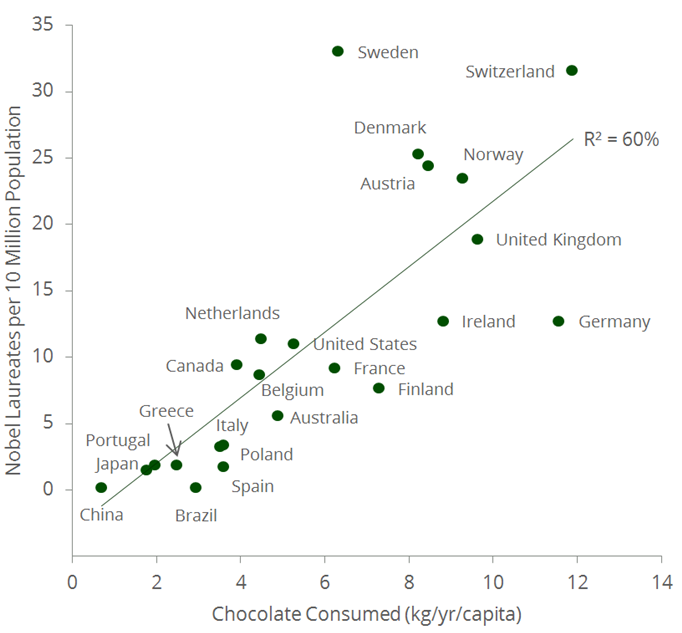
\includegraphics[width=0.7\textwidth]{Chocolate_consumption.png}
    \caption{Конзумација чоколаде и добитници Нобелове награде. Преузето са: \textit{https://www.dectech.co.uk/news-insights/buzz/why-is-correlation-not-causation-part-i/}}
    \label{fig:uzrocnost}
\end{figure}

Да бисмо избегли оваква погрешна тумачења, важно је јасно разграничити шта је корелација, а шта каузалност и разумети на који начин се ови односи испитују у статистици.

Корелација и каузалност представљају две различите врсте односа између променљивих. Корелација описује статистичку повезаност: две променљиве се крећу заједно на 
предвидљив начин, али то не значи да промена једне узрокује промену друге. Каузалност, с друге стране, подразумева да промена једне променљиве директно доводи до 
промене друге, при чему постоји стварна узрочна веза. Док корелација мери само обрасце заједничког кретања података, каузалност захтева разумевање механизма који 
повезује променљиве и обично укључује контролу других фактора који могу утицати на посматрани однос.

Корелација представља најнижи ниво каузалне хијерархије и дефинише се поређењем очекиваног исхода код тренираних и нетретираних у стварном свету, $E[Y|A=1] \neq E[Y|A=0]$.
Каузалност подразумева поређење целокупне популације када би сви били третирани, $E[Y^{a=1}]$, са исходом када би сви били нетретирани, $E[Y^{a=0}]$.
Корелација може постојави чак и када међу њима нема каузалне везе, обично због постојања заједничког узорка.
Принцип заједничког узрока формализује ове могућности: ако су две случајне променљиве $X$ и $Y$ статистички 
зависне, онда је могуће да 
\begin{enumerate}
    \item $X$ узрокује $Y$
    \item $Y$ узрокује $X$
    \item постоји трећа променљива $Z$ која узрокује и $X$ и $Y$, при чему $X$ и $Y$ постају независне ако се узме у обзир $Z$
\end{enumerate}
Каузално закључивање пружа алате који нам омогућавају да донесемо узрочне закључке чак и у одсуству истинског експеримента, под условом да су испуњене
одређене претпоставке (условна заменљивост, позитивност и конзистентност) о којима ће бити речи касније. 

Да би се боље разумела практична важност каузалног закључивања, корисно је погледати како оно функционише у стварним истраживачким ситуацијама и како помаже да се 
избегну погрешни закључци засновани само на корелацији.

\subsubsection{Главне разлике, истраживања, илустрација примером}
Каузално закључивање је важно, на пример, у медицинским истраживањима једна група може добијати плацебо, док друга добија нови тип лека.
Ако се исходи између те две групе значајно разликују, управо различита искуства могу бити узрок тих различитих исхода.

Поред експерименталних дизајна, каузално размишљање је кључно и код анализа опсервационих података. Један од феномена који најбоље илуструје ову потребу јесте 
Симпсонов парадокс.

Симпсонов парадокс представља појаву у којој се однос између две променљиве мења или чак потпуно преокреће када се подаци 
посматрају у целини у односу на њихове подгрупе. Другим речима, корелација која важи на агрегатном нивоу може нестати или 
се обрнути када се подаци разбију по релевантним категоријама.

Овај парадокс јасно показује зашто „корелација не повлачи узрочност“ – наизглед јака веза може бити последица прикривених 
(конфаундирајућих) фактора. %ovde dodati i primer sa doktorima
Класичан пример је анализа успеха лечења код мушкараца и жена: када се посматрају подаци укупно, 
једна терапија делује успешније, док када се подаци раздвоје по полу, испостави се да је друга терапија боља у обе групе.

Суштина Симпсоновог парадокса је у томе да исту корелацију можемо тумачити потпуно другачије у зависности од нивоа анализе. 
Због тога се у каузалном закључивању наглашава важност идентификације и контроле скривених променљивих како би се избегли 
погрешни закључци.

Разликовање корелације и каузалности је само први корак ка разумевању узрочних односа. Да бисмо могли прецизније да објаснимо и измеримо ефекте различитих интервенција, 
потребан нам је формалнији оквир. У наставку ће бити представљени кључни појмови као што су контрафактуални исходи, просечни третмански ефекат (ATE), претпоставка 
SUTVA и Рубинов каузални модел, који нам помажу да каузално размишљање претворимо у конкретне статистичке алате.


\subsection{Фундаментални проблем}
    \subsubsection{Рубинов каузални модел}
    \subsubsection{АТЕ (Average Treatment Effect), дефиниција}
    \subsubsection{проблем контрафактуала, немогућност да посматрамо оба света истовремено}
\subsection{Математичке основе иза концепта узрочности}
    \subsubsection{АТЕ (процена и математичке импликације)}
    \subsubsection{СУТВА}
    \subsubsection{алгоритми за процену ефекта}
\subsection{Утврђивање кауланости и експерименти (прелазак на следеће поглавље)}

\newpage



\section{Рандомизирани експеримент}
\newpage



\section{Опсервационе студије}


\end{document}

